\section{Information about difficult structures}
\begin{center}
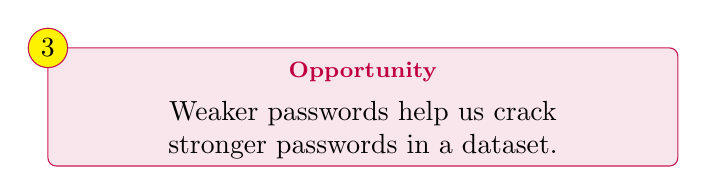
\begin{tikzpicture}
    \def\gridwidth{8}
    \def\gridheight{1.5}

    % Draw the main grid
    \draw[fill=purple!10, draw=purple!90, rounded corners=3pt,] (0,0) rectangle (\gridwidth,\gridheight);

    \node[align=center, text=purple, font=\footnotesize] (box1) at (\gridwidth/2,\gridheight-0.3) {\bf Opportunity};
        
    \node[below, text width=7cm, align=center] at (box1.south) {Weaker passwords help us crack stronger passwords in a dataset.};
    
    \node[circle,fill=yellow,inner sep=0pt,minimum size=0.5cm, draw=purple!90] at (0,\gridheight) {3};
\end{tikzpicture}
\end{center}

To formalise the expected information gain about words in $wwww$ or $\bm{w^4}$ structures given knowledge of words used in `w`, we utilise concepts from information theory, specifically entropy and conditional entropy. This approach quantifies the uncertainty in the $\bm{w^4}$ structures and how this uncertainty is reduced with knowledge of the `w` distributions.

Maximise expected information gain from cracking a certain structure.

\subsection*{Entropy}

Entropy (\(H\)) measures the unpredictability or randomness of a system. For a set of words \(W\), the entropy is calculated as:

\[
H(W) = -\sum_{i=1}^{n} P(w_i) \log_2 P(w_i)
\]

where \(P(w_i)\) is the probability of the \(i^{th}\) word occurring in the set, and \(n\) is the number of unique words.

\subsection*{Conditional Entropy}

Conditional entropy (\(H(W|W')\)) measures the amount of uncertainty remaining about \(W\) (the words in `wwww`) given \(W'\) (the distribution of words in `w`). It's defined as:

\[
H(W|W') = -\sum_{j=1}^{m} P(w'_j) \sum_{i=1}^{n} P(w_i|w'_j) \log_2 P(w_i|w'_j)
\]

where \(P(w_i|w'_j)\) is the conditional probability of word \(w_i\) given the word \(w'_j\), \(m\) is the total number of `w` words, and \(n\) is the total number of `wwww` structures.

\subsection*{Expected Information Gain}

The expected information gain (\(IG\)) about the words in `wwww` structures given knowledge of `w` can be calculated as the difference between the initial entropy of `wwww` and the conditional entropy of `wwww` given `w`:

\[
IG(W;W') = H(W) - H(W|W')
\]

This quantifies how much knowing the distribution of single words (`w`) reduces our uncertainty about the composition of phrases (`wwww`).

\subsection*{Applying the Formalization}

1. \textbf{Calculate \(H(W)\)}: Compute the entropy of the `wwww` structures based on their distribution. This involves analyzing the dataset to determine the probability distribution of different `wwww` structures.

2. \textbf{Calculate \(H(W|W')\)}: Compute the conditional entropy of `wwww` given `w`. This requires understanding how likely each `w` word is to appear in the `wwww` structures.

3. \textbf{Compute \(IG(W;W')\)}: Calculate the expected information gain, indicating how much knowing `w` aids in predicting `wwww`.

\subsection*{Practical Considerations}

- \textbf{Probability Estimation}: Estimating \(P(w_i)\) and \(P(w_i|w'_j)\) necessitates a thorough analysis of the dataset, considering both `w` and `wwww` distributions.

- \textbf{Complexity}: The actual combinations of `w` into `wwww` and their probabilities can be complex, requiring a detailed understanding of language patterns.

- \textbf{Data Requirements}: Accurate estimation of these probabilities and the information gain requires a large and representative dataset of both `w` and `wwww`.
